% !TEX root = ../Main.tex

\subsection{Atomistix ToolKit: ATKPython and Nanolanguage}
In this project we will utilise the Atomistix ToolKit, developed by QuantumWise\footnote{\url{https://quantumwise.com/}}, or ATK for short. The Toolkit takes Python scripts as inputs and simulates a completely custom lattice enviroment with various applied calculations. It is possible to simulate very specific scenarios, alter the simulation parameters and extract results for analysis easily and fast.
\subsubsection{Nanolanguage}
ATKPython (the standalone simulation program) extends the Python language with Nanolanguage which tells ATKPython what to do when launched. One can set up specific bravais lattices and repeat them into large 2D structures. Then specific atoms can be tagged or altered and calculations can be set up. All of these features are available through QuantumWise VNL, a GUI which sets up the scripts and calculations, if need be. The GUI is shown on \cref{VNLLAB}
\begin{figure}
 \centering
 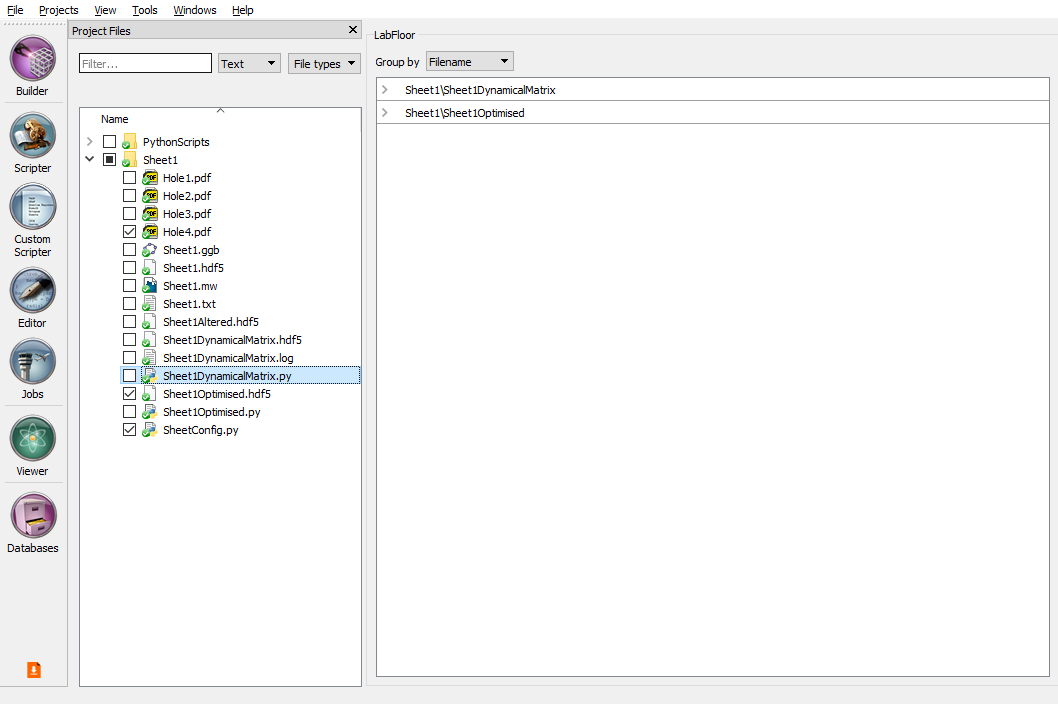
\includegraphics[width=\columnwidth]{Figures/VNLLabfloor.png}
 \caption{The VNL Labfloor user interface shows project files in the center frame and various tools in the left pane.}
 \label{VNLLAB}
\end{figure}
\subsubsection{VNL and ATK workflow}
The workflow for running simulations is described below:
\begin{enumerate}
 \item Create lattice
 \item (optional) Alter lattice with text editor
 \item Specify calculators
 \item (optional) Alter calculation parameters and output files with text editor
 \item Run simulations
 \item (optional) Extract data with ATKPython
 \item Analyse with built-in tools
\end{enumerate}
\subsubsection{NanoSheetCreator.py}
In this project Nanolanguage will largely be used to alter crated simulation scripts, made with the VNL GUI, before using ATKPython, however a script for creating the Graphene lattice with specifically sized hexagonal holes has been written to effectively creating various lattices. The script makes a hexagonal bravais lattice and tags atoms at a specific location and in a custom sized hexagonal shape. The the script can repeat this setup as many times along the generating vectors.

First the script creates a bravais-lattice consisting of a hexagonal unit cell. Then two carbon atoms are placed in the unitcell and the unit cell is repeated to the users specifications.
\onecolumngrid


\begin{listing}
    \inputminted[python3=true,bgcolor=Black,linenos=true,firstline=24,lastline=35]{python}{VNL/PythonScripts/NanoSheetCreator.py}
    \caption{Lines 24-35 from the NanoSheetCreator.py shows how    Nanolanguage can be used to create a hexagonal bravais lattice}
    \label{listing1}
\end{listing}
\twocolumngrid
The script prints information about the size of the sheet and the user is asked to input position and size of the hexagonal tag wanted. One can save the sheet and tag as a figure before adding more tags. Lastly the sheet can be repeated and information about the position and sizes of the tags are printed to a \textit{.txt} file.

The Python script creating the lattice and tags are printed and commented in the Appendix on \cpagerefrange{NSCstart}{NSCend}
